\documentclass[a4paper,twoside]{scrartcl}

\usepackage[ngerman]{babel}
\usepackage[final]{microtype}
\usepackage[T1]{fontenc}
\linespread{1.05}

\usepackage[inner=3cm,outer=2cm,top=3cm,bottom=3cm,foot=1.75cm]{geometry}
\setlength{\columnsep}{20pt}

\usepackage{xcolor}
\usepackage{lmodern}
\usepackage{amsmath, amsthm, amssymb, mathtools}
\usepackage{unicode-math}
\usepackage{fontspec}
\defaultfontfeatures{Ligatures=TeX,Scale=MatchLowercase}

\let\emptyset\varnothing

\usepackage{url}
\usepackage{graphicx}

\usepackage{enumitem}
\setlist{nolistsep}
\setlist[itemize]{noitemsep}

\setlength{\parindent}{0pt}
\setlength{\parskip}{6pt plus 2pt minus 1pt}

\usepackage[font=small]{caption}

\usepackage{abstract}
\renewcommand{\abstractnamefont}{\normalfont\bfseries}
\renewcommand{\abstracttextfont}{\normalfont\small}

\usepackage{titlesec}
\renewcommand\thesection{\Roman{section}}
\renewcommand\thesubsection{\roman{subsection}}
\titleformat{\section}[block]{\large\scshape\centering}{\thesection.}{1em}{}
\titleformat{\subsection}[block]{\large}{\thesubsection.}{1em}{}

\usepackage{hyperref}
\hypersetup{pdfborder={0 0 0},breaklinks=true}

\setlength{\emergencystretch}{3em}
\interfootnotelinepenalty=10000

\usepackage{titling}
\setlength{\droptitle}{-2\baselineskip}
\pretitle{\begin{center}\huge\bfseries}
\posttitle{\end{center}}
\renewcommand{\subtitle}[1]{%
  \posttitle{%
    \par\end{center}
    \begin{center}\Large\bfseries#1\end{center}
    \vskip0.5em}%
}

\usepackage[automark]{scrpage2}
\pagestyle{scrheadings}
\clearscrheadfoot
\rohead[]{\textsc{\leftmark}}
\lehead[]{\textsc{\leftmark}}
\rofoot[\pagemark]{\pagemark}
\lefoot[\pagemark]{\pagemark}

\makeatletter
  \newcommand\footnoteref[1]{\protected@xdef\@thefnmark{\ref{#1}}\@footnotemark}
\makeatother

\renewcommand{\arraystretch}{1.2}

\renewcommand{\maketitlehookd}{%
  \vspace{\baselineskip}
  \begin{abstract}
  \noindent Was sind Spielbäume und wozu können sie verwendet werden? In dieser Ausarbeitung wird das Konzept des Spielbaumes formal eingeführt und anhand des Spiels \e{Tic-Tac-Toe} beispielhaft erläutert. Mit der Erklärung des Alpha-Beta-Prunings als Optimierung des Minmax-Verfahrens und anderer Heuristiken wird eine Anwendung von Spielbäumen illustriert.
  \end{abstract}
  \vspace{\baselineskip}
}

\newcommand\e[1]{\begin{em}#1\end{em}}

\newcommand\q[1]{\glqq #1\grqq}

\newcommand\sq[1]{\glq #1\grq}

\newcommand\qq[1]{\glqq\e{#1}\grqq}

\newcommand\fnm[1]{\footnotemark[#1]\addtocounter{footnote}{1}}

\newcommand\g[4]{%
  \begin{figure}[!ht]
  \centering
  \includegraphics[width=#4\textwidth]{#1}
  \caption{#3\label{fig:#2}}
  \end{figure}}

\newcommand\todo[1]{\colorbox{yellow}{#1}}


\title{Spielbäume}
\def\titlehead{Spielbäume}
\subtitle{Proseminar Theoretische Informatik}
\author{Joschka Heinrich\thanks{joschka.heinrich@tu-dresden.de, PGP: \textsc{B40E 67C7 FF62 C860 7854 A778 6FB9 666F 1147 A401}}, TU Dresden}

\begin{document}
\maketitle



\section{Einführung}
\todo{Motivation. Überblick Aufbau Text.}



\section{Spielbäume}
Um im Folgenden mit Spielbäumen arbeiten zu können, führen wir das Konzept zunächst formal ein und definieren dazu unter anderem den Begriff des \e{Spiels}, der \e{Konfiguration} und des \e{Spielbaums}.


\subsection{Definition}

\todo{Nullsummenspiel}

Alle folgenden Betrachtungen nehmen wir aus der Perspektive eines gewinnorientierten Spielers namens \textsc{Max} vor, der sich einer Anzahl Gegner gegenüber sieht. Es ist also das Ziel, Züge für \textsc{Max} so zu finden, dass dessen Gewinn maximiert, bzw. der Gewinn der Gegner minimiert wird. Wir gehen dabei davon aus, dass auch alle Gegner optimale Entscheidungen treffen. Wir vereinfachen die Betrachtung von Spielen, indem wir uns auf solche ohne Zufallskomponente, d.h. reine Strategiespiele mit vollkommener Information und Spiele mit zwei Kontrahenten -- \textsc{Max} und ein zweiter Spieler \textsc{Min} -- beschränken. Mit \q{der Gegner} ist also im Folgenden stets \textsc{Min} gemeint. 

Ein \textbf{Spiel} $S = (R,k_0,F)$ ist nun durch Regeln, in Form einer endlichen Menge von legalen Spielzügen $R$, eine Anfangskonfiguration $k_0 \in K$ und eine Reihe möglicher Endkonfigurationen $F \subset K$ gegeben, mit $K$, der Menge aller \e{zulässigen} Konfigurationen. Eine \textbf{Konfiguration} $k \in K$ repräsentiert dabei einen möglichen Zustand des Spieles, bestehend aus einer Beschreibung wiederum der Zustände aller relevanten Spielelemente (bspw. die Position der Zeichen auf dem Tic-Tac-Toe-Feld) inklusive des Spielers, der als nächster an der Reihe ist (bei uns entweder \textsc{Max} oder \textsc{Min}).

In Abgrenzung zur Menge der \e{legalen} Spielzüge können wir uns beliebige andere Spielzüge vorstellen, die zwar möglich, allerdings in dem betrachteten Spiel nicht erlaubt sind. Analog dazu sind über $K$ hinaus weitere Konfigurationen denkbar, die allerdings nicht zulässig sind, d.h. in einem regelkonformen Spiel niemals auftreten können. Durch Anwenden eines legalen Spielzuges auf eine Konfiguration gelangen wir zu einer neuen Konfiguration. Dieser Zusammenhang wird in Abb.~\ref{fig:venn} veranschaulicht. Ein legaler Spielzug kann also als eine Funktionen $R:K \to K$ verstanden werden. Seien $u,v \in K$ Konfigurationen und $r \in R$ ein legaler Spielzug, mit $v = r(u)$, dann heißt $v$ \textbf{Kindkonfiguration} von $u$ (bezüglich $r$) und $u$ \textbf{Elternkonfiguration} von $v$ (bezüglich $r$). 

\g{img/spielzuege.pdf}{venn}{Das \textsc{Venn}--Diagramm zeigt die Teilmengenbeziehungen der Spielzüge einerseits und der Konfigurationen andererseits, wobei $K$ induktiv über $R$ definiert ist.}{.9}

Wenn das Anwenden eines Spielzuges zu einer neuen Konfiguration führt, also $u \neq v$ gilt, dann heißt $r$ \textbf{anwendbar} auf u.\footnote{Das bedeutet nicht notwendigerweise, dass sich die Konfiguration der Spielelemente verändert. Zwei Spielkonfigurationen können sich auch darin unterscheiden, welcher Spieler an der Reihe ist.} Gibt es mehrere auf eine Konfiguration $k \in K$ anwendbare Spielzüge, erhalten wir eine \textbf{Menge von Kindkonfigurationen} $N(k) \subset K$ mit $N(k) = \{r(k) \mid r \in R,~r \textrm{ anwendbar auf } k\}$. Auf eine Endkonfiguration $k_f \in F$ sind keine Spielzüge anwendbar, da das Spiel mit Erreichen einer dieser Konfigurationen als beendet gilt: $N(k_f) = \emptyset$.

Die Menge $K$ definieren wir nun induktiv über die Kindkonfiguration: 
\begin{itemize}
	\item $k_0$ ist Element von $K$.
	\item Wenn $k \in K$, dann auch alle $k' \in N(k)$.
\end{itemize}

Alle zulässigen Konfigurationen lassen sich also aus der Anfangskonfiguration und den legalen Spielzügen ableiten. Zu jeder Konfiguration $k \in K \setminus F$ gehört eindeutig eine Menge von Kindkonfigurationen $N(k)$ und zu jeder Konfiguration $k \in K \setminus k_0$ eine Elternkonfiguration $k'$. Diese Beziehungen können durch einen Graphen anschaulich dargestellt werden.

Ein \textbf{Spielgraph} ist ein gerichteter Graph $G(V,E)$ mit: 
\begin{itemize}
	\item Knoten $V = K$ und
	\item Kanten $E = \bigcup\limits_{u \in K}\{(u,v) \mid v \in N(u)\}$
\end{itemize}

Als zusätzliche Vereinfachung schließen wir aus, eine über $R$ aus $k_0$ generierte Konfiguration durch erneutes Anwenden legaler Spielzüge wieder erreichen zu können. Wir gelangen also im weiteren Spielverlauf nie zu einer Situation, die bereits aufgetreten ist.\footnote{Diese Einschränkung schließt viele Spiele wie bspw. Schach von der folgenden Betrachtung aus, da dort durch legale Spielzüge Konfigurationen reproduziert werden können. Viele der Aussagen lassen sich dennoch auch auf diese Art Spiele übertragen.} Daraus folgt unmittelbar, dass $G$ zyklenfrei ist.

Damit ist der Graphen $G$ insbesondere ein Baum\footnote{\label{suchbaum}Wir benutzen also im Folgenden -- abweichend der Terminologie der Hauptquelle\cite{klueppel:2016} -- , mit den hier getroffenen Annahmen, \q{Spielgraph} synonym zu \q{Spielbaum}. Davon abzugrenzen ist der Begriff \q{Suchbaum}. Während der \e{Spielbaum} ein theoretisches Modell von großer (Speicher-)Komplexität ist, wird der \e{Suchbaum} zur Laufzeit generiert und bildet kein vollständiges Spiel ab.}, mit $k_0$ als Wurzel und $F$ als Blätter. So kann über den Baum entlang legaler Spielzüge traversiert werden und bspw. ein kompletter Spielverlauf mit $n$ Zügen als Pfad $(k_0, k_1, \dots, k_n \in F)$ subsequenter Kindkonfigurationen dargestellt werden.


\subsection{Am Beispiel Tic-Tac-Toe}

Um obige Definitionen zu veranschaulichen, wenden wir sie nun auf das Spiel Tic-Tac-Toe an. Das Tic-Tac-Toe-Spielfeld besteht aus einem $3 \times 3$-Raster mit neun Feldern in die zwei Spieler abwechselnd ihre Zeichen setzen. Dies sind üblicherweise \q{X} bzw. \q{O}. Im Folgenden wird \textsc{Max} mit \q{X} und \textsc{Min} mit \q{O} spielen.

Ziel jedes Spielers ist es, drei der eigenen Zeichen nebeneinander zu setzen, d.h. in einer Reihe, Spalte oder Diagonale, und gleichzeitig zu verhindern, dass der Gegner seine Zeichen in dieser Weise setzen kann. Das Spiel endet entweder, wenn einer der beiden Spieler gewinnt, sobald er dieses Ziel erreicht, oder wenn kein Zug mehr möglich ist, da alle neun Felder belegt sind. Das Spiel geht in diesem Fall unentschieden aus.

\g{tic.pdf}{tictactoe}{Ein Tic-Tac-Toe-Spielbaum der Tiefe 2, bei dem die Anzahl der Konfigurationen bereits durch Ausnutzung von Symmetrien optimiert wurde.}{.9}

\section{Zugplanung}

Es stellt sich nun die Frage, wie sich aus den bekannten möglichen Zügen, die sich aus einer Spielsituation ergeben, der beste Zug auswählen lässt. \textsc{Max} wählt seine Züge stets so, dass sein Vorteil maximiert wird, wenn er am Zug ist. Da angenommen wird, dass \textsc{Min} genauso handelt, heißt das auch, dass er jenen Zug von \textsc{Min} antizipieren muss, der ihm den größten Nachteil bringen wird.\footnote{In Anlehnung an \cite{russel:2012} tragen \textsc{Max} und \textsc{Min} auch genau aus diesem Grund ihre Namen: ist \textsc{Max} an der Reihe, wird der Nutzen \textit{maximiert}; ist es \textsc{Min}, wird er \textit{minimiert}; stets aus der Sicht von \textsc{Max}.}. Dieses Vorgehen führt zum \textbf{Minmax-Verfahren}\footnote{erstmals 1912 von \textsc{E. Zermelo} erwähnt, 1913 veröffentlicht\cite{zermelo:1913}}, das wir im Folgenden genauer betrachten. Auch werden wir einige dessen Optimierungen kennenlernen, um unvollständige Echtzeitentscheidungen treffen zu können.


\subsection{Minmax-Verfahren}

Zunächst führen wir eine \textbf{Gewinnfunktion} $g: F \to \mathbb{N}$ ein, die die Blätter des Spielbaumes bewertet und ihnen einen Wert zuordnet, wie günstig dieser Ausgang für \textsc{Max} wäre.

Des Weiteren benötigen wir zwei Typen von Knoten in unserem Spielbaum: \textbf{Max-Knoten} (im folgenden mit $\bigtriangleup$ gekennzeichnet), an denen \textsc{Max} am Zug ist und der Nutzen maximiert werden soll und analog dazu \textbf{Min-Knoten} ($\bigtriangledown$). In unserem Tic-Tac-Toe-Szenario alternieren die Knoten-Typen mit jedem Halbzug\footnote{Ein Zug entspricht einer Runde, in der sowohl \textsc{Max} und \textsc{Min} einmal an der Reihe waren und besteht aus zwei Halbzügen.}, da die Spieler sich stets abwechseln. 

Jedem Knoten $u$ im Spielbaum wird nun ein \textbf{Minmax-Wert} $minmax(u) \in \mathbb{N}$, der dem Nutzen aus Sicht von \textsc{Max} entspricht, zugeordnet. Dabei ergibt sich $minmax(u)$ rekursiv aus den Minmax-Werten der Kindknoten $N(u)$ und kann wird mit einer Tiefensuche\footnote{Als zusätzliche Optimierung, die sich auch aus weiteren Gründen anbietet, wie wir sehen werden, bietet sich dafür in der Praxis die Verwendung der \textit{iterativen Tiefensuche} an.} wie folgt rekursiv berechnet:
\[
  minmax(u) = \left\{
  \begin{tabular}{cl}
    $g(u)$ & wenn $u \in F$\\
    $\max\limits_{v \in N(u)} minmax(v)$ & wenn $u$ Max-Knoten\\
    $\min\limits_{v \in N(u)} minmax(v)$ & wenn $u$ Min-Knoten
  \end{tabular}\right.
\]

Die Rekursion endet mit dem Erreichen einer Endkonfiguration, dann wird die Gewinnfunktion angewendet. Je nach dem in welcher Ebene (Min oder Max) des Baumes wir uns befinden wird beim folgenden Aufstieg entsprechend das Minimum bzw. Maximum der Kinder nach oben weitergegeben. Schließlich wählt \textsc{Max} den Zug mit dem größten Minmax-Wert als seinen nächsten Zug. (vgl. Abb.~\ref{fig:minmax})

\g{img/tic_minmax_2.pdf}{minmax}{Ein Ausschnitt eines hypothetischen Spielbaumes an dem das Prinzip des Minmax-Verfahrens nachvollzogen werden kann: eine Gewinnfunktion bewertet Endkonfigurationen mit $1$ bei Gewinn, $-1$ bei Niederlage und $0$ bei Unentschieden; die Minmax-Werte werden entsprechend des Algorithmus' bis zur Wurzel propagiert; \textsc{Max} wählt schließlich den ersten Zug mit dem Kreuz in der Mitte, da der Minmax-Wert hier maximal ist.}{.4}

Würde wir tatsächlich den gesamten Spielbaum mit diesem Verfahren durchsuchen, ergibt sich mit der maximalen Tiefe $m$ des Baumes und einem Verzweigungsgrad $b$ eine Zeitkomplexität von $\mathcal{O}(b^m)$ sowie eine Speicherkomplexität von $\mathcal{O}(bm)$. Die Speicherkomplexität beträgt lediglich $\mathcal{O}(m)$, wenn nur der aktuelle Pfad im Speicher gehalten wird. Ohne Optimierungen müsste der Baum vollständig durchlaufen werden. Da schon bei sehr einfachen Spielen wie Tic-Tac-Toe, mit wenigen Freiheiten und einer überschaubaren Zuganzahl, die Anzahl der möglichen Konfigurationen zu groß wird, um in annehmbarer Zeit Züge zu berechnen\footnote{Der Tic-Tac-Toe-Spielbaum hat ohne Optimierung $9! = 362880$ Knoten, obwohl es \q{nur} $5478$ verschiedene Konfigurationen gibt, die sich allerdings in insgesamt $255168$ möglichen Spielverläufen wiederholen. (Ein Spiel kann auch schon mit weniger als 9 Zügen beendet werden.) Unter Ausnutzung von Symmetrien erhalten wir $765$ Konfigurationen und $31896$ Spielverläufe.}, kann das Verfahren so nicht angewendet werden. Vor allem bei Agenten für wesentlich komplexere und längere Spiele, wie Schach, kommen daher unter anderem folgende Optimierungen zum Einsatz.


\subsection{Optimierung mittels Heuristik}
Damit nicht mehr der gesamte (und potenziell sehr tiefe) Teil-Baum der Kindkonfigurationen rekursiv bis zu den Blättern durchsucht werden muss, um die Minmax-Bewertung eines Knotens $k$ weiter oben im Baum zu erhalten, führen wir nun eine \textbf{Heuristik} ein. Diese ermöglicht es, auch nicht-Endkonfigurationen einen \textit{geschätzten} Nutzen zuzuordnen, basierend auf Merkmalen der Konfiguration. Der Spielbaum muss dann nur noch in einer festen Suchtiefe $t$ analysiert werden.\footnote{Bisher haben wir so lange Knoten expandiert, d.h. deren Kinder analysiert, bis eine Endkonfiguration erreicht war (im Fall des Spielbaumes, da nur eine Gewinnfunktion zur Verfügung stand). Da mit der Heuristik nun jede Konfiguration bewertet werden kann, ist dies nicht mehr nötig. Es stellt sich allerdings die Frage nach einem guten \textbf{Expansionskriterium}; d.h., wann es sinnvoll ist, einen Knoten noch weiter zu expandieren. Wir arbeiten hier weiter mit dem Kriterium einer festen Suchtiefe $t$, allerdings lassen sich weitere Expansionskriterien finden, die zu besseren Entscheidungen führen können. Die Suchtiefe kann auch über den Spielverlauf hinweg variiert werden.} Den Baum, den wir ausgehend von einer beliebigen Konfiguration des Spielbaumes in der Tiefe $t$ zur Laufzeit effizient aufbauen nennen wir \textbf{Suchbaum} (siehe dazu auch \footnoteref{suchbaum}).

Diese Heuristik $h(k)$ muss (1) die gleiche Ordnung wie die Gewinnfunktion $g(k)$ erzeugen, d.h. ebenso einen Gewinn besser als ein Unentschieden und dieses besser als eine Niederlage werten. Sie muss (2) effizient sein, sonst ist die Optimierung nicht sinnvoll, und muss (3) möglichst genau sein, d.h. Werte für nicht-Endkonfigurationen schätzen, die möglichst nah am tatsächlichen Nutzen liegen.

Eine Heuristik für Tic-Tac-Toe könnte bspw. mit $h_1(k) = A_X(k) - A_O(k)$ definiert werden, wobei $A_{X}$ bzw. $A_{O}$ jeweils die Summe an möglichen Horizontalen, Vertikalen und Diagonalen bezeichnet, die mit drei der entsprechenden Zeichen (\q{X} oder \q{O}) vervollständigt werden könnten. (s. Abb.~\ref{fig:heuristic})

\begin{figure}[!ht]
  \centering
  \begin{tabular}{ll}
    (a) & 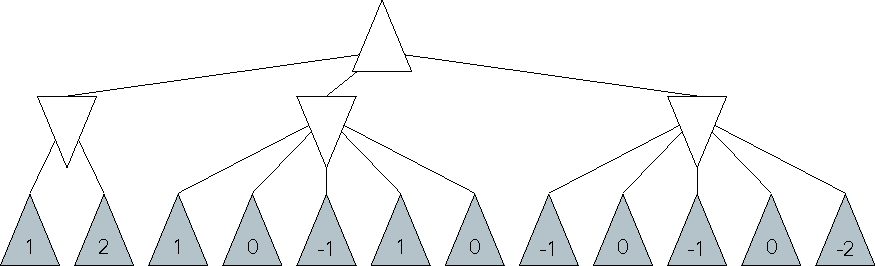
\includegraphics[width=.8\textwidth]{minmax_heuristik.pdf}\\
        & \\
    (b) & 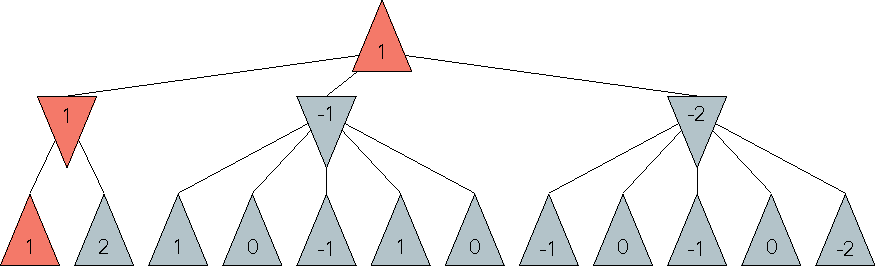
\includegraphics[width=.8\textwidth]{minmax_heuristik_2.pdf}
  \end{tabular}
  \caption{Wenden wir einen Suchbaum der Suchtiefe $t = 2$, ausgehend von der Startkonfiguration des leeren Feldes, aufbauen (vgl. Abb.~\ref{fig:tictactoe}) und dessen Blätter mit der Heuristik $h_1$ bewerten, erhalten wir die geschätzten Werte aus (a), die in (b) im gewohnten Modus zur Wurzel propagiert werden. Der Zug den \textsc{Max} wählt ist hervorgehoben.\label{fig:heuristic}}
\end{figure}


\subsection{Alpha-Beta-Pruning}

Um die Komplexität des Minmax-Algorithmus weiter zu verringern, nehmen wir eine weitere Optimierung vor: das \textbf{Alpha-Beta-Pruning}\footnote{erstmals 1956 vorgestellt (\textsc{McCarthy}), auch \q{Alpha-Beta-Kürzung}, \q{$\alpha$-$\beta$-Pruning}, \q{$\alpha$-$\beta$-Cut} oder \q{$\alpha$-$\beta$-Suche}}. Dieses erlaubt es, das Untersuchen von Teilbäume abzukürzen, ohne dabei gute Züge auszuschließen, indem Knoten nicht weiter expandiert werden, auch, wenn das Expansionskriterium erfüllt ist. 

Dazu führen wir für jeden Knoten $k$ zusätzlich einen \textbf{Alpha-} und \textbf{Beta-Wert} $\alpha_k$ und $\beta_k$ ein. $\alpha_k$ ist dabei die \textit{untere} Schranke des Minmax-Wertes $minmax(k)$ für Max-Knoten und speichert die bisher \textit{größte} Bewertung im Pfad von der Wurzel des aktuellen Suchbaumes zum Knoten $k$. Analog wird in $\beta_k$ die \textit{obere} Schranke für Min-Knoten gespeichert, d.h. die bisher \textit{kleinste} Bewertung im Pfad zu $k$.

Die Alpha- und Beta-Werte werden mit $\alpha = -\infty$, $\beta = +\infty$ initialisiert und nach jeder untersuchten Konfiguration aktualisiert, so dass $\alpha$ an einem Max-Knoten stets maximiert und $\beta$ an einem Min-Knoten stets minimiert wird.

Wir können nun auf Basis der $\alpha$ und $\beta$ Werte \textbf{Kürzungen (Cut)} vornehmen, d.h. Teilbäume aus dem Suchbaum löschen, sobald sich die beiden Schranken überschneiden: An einem Max-Knoten $u$ -- es wird hier stets der größte Minmax-Wert unter den Kindknoten gesucht --  führen wir den s.g. \textbf{$\alpha$-Cut} durch, sobald $\exists \beta_v : \beta_v \leq \alpha_u$ ($v \in N(u)$). Analog dazu wird der \textbf{$\beta$-Cut} an einem Min-Knoten durchgeführt, wenn $\exists \alpha_v : \alpha_v \geq \beta_u$ ($v \in N(u)$).


\todo{Beispiel, Grafik, Komplexität}


\section{Zusammenfassung}

\todo{Schlussfolgerung. Ausblick. Anwendbarkeit, Zufallsspiele}


\begin{thebibliography}{99}
  \bibitem{klueppel:2016} \textsc{Sascha Klüppelholz}
  \newblock \q{Entwurfs- und Analysemethoden für Algorithmen -- Skript zur Vorlesung}, Sommersemester 2016
  \bibitem{russel:2012} \textsc{Russel, Norvig}
  \newblock \q{Künstliche Intelligenz -- Ein moderner Ansatz}, 3., aktualisierte Auflage, 2012
  \bibitem{zermelo:1913} \textsc{Ernst Zermelo}
  \newblock \q{Über eine Anwendung der Mengenlehre auf die Theorie des Schachspiels}, 1913
\end{thebibliography}


\vspace{4\baselineskip}
Diese Ausarbeitung und zugehörige Präsentation sind auch auf github zu finden: \\\url{https://github.com/foobar0112/tic}.

\end{document}